
\chapter{Proof techniques II --- Induction}


\section{The principle of mathematical induction}
\label{sec:induct}


\noindent{\large \bf Exercises --- \thesection\ }

\begin{enumerate}
\item Consider the sequence of number that are 1 greater than a multiple of 4.
(Such numbers are of the form $4j+1$.)

\[ 1, 5, 9, 13, 17, 21, 25, 29, \ldots \]

The sum of the first several numbers in this sequence can be expressed as
a polynomial.

\[ \sum_{j=0}^n 4j+1 = 2n^2 + 3n + 1 \]

Complete the following table in order to provide evidence that the formula
above is correct.

\begin{center}
\begin{tabular}{c|c|c}
$n$ & $\sum_{j=0}^n 4j+1$ & $2n^2 + 3n + 1$ \\ \hline
 0 & $1$ & $1$ \\
 1 & $1 + 5 = 6$ &  $2 \cdot 1^2 + 3 \cdot 1 + 1 = 6$ \\
 2 & $1 + 5 + 9 = \rule{15pt}{0pt}$ & \\
 3 & & \\
 4 & & \\
\end{tabular}
\end{center}



\item \label{ex:horses} What is wrong with the following inductive proof of
``all horses are the same color.''?

{\bf Theorem} Let $H$ be a set of $n$ horses, all horses in $H$ 
are the same color.

\begin{proof}
We proceed by induction on $n$.

\noindent {\bf Basis: } Suppose $H$ is a set containing 1 horse.  Clearly
this horse is the same color as itself.

\noindent {\bf Inductive step: } Given a set of $k+1$ horses $H$ we can 
construct two sets of $k$ horses.  Suppose $H = \{ h_1, h_2, h_3, \ldots h_{k+1} \}$.  Define $H_a = \{ h_1, h_2, h_3, \ldots h_{k} \}$ (i.e. $H_a$ contains
just the first $k$ horses) and $H_b = \{ h_2, h_3, h_4, \ldots h_{k+1} \}$ 
(i.e. $H_b$ contains the last $k$ horses).  By the inductive hypothesis
both these sets contain horses that are ``all the same color.''  Also,
all the horses from $h_2$ to $h_k$ are in both sets so both $H_a$ and
$H_b$ contain only horses of this (same) color.  Finally, we conclude that
all the horses in $H$ are the same color.

\end{proof}
\medskip
   
\item For each of the following theorems, write the statement that must be
proved for the basis -- then prove it, if you can!

\begin{enumerate}
\item The sum of the first $n$ positive integers is $(n^2+n)/2$.
\item The sum of the first $n$ (positive) odd numbers is $n^2$.
\item If $n$ coins are flipped, the probability that all of them 
are ``heads'' is $1/2^n$
\item Every $2^n \times 2^n$ chessboard -- with one square removed -- can 
be tiled perfectly\footnote{Here, ``perfectly tiled'' means that every trominoe
covers 3 squares of the chessboard (nothing hangs over the edge) and that every
square of the chessboard is covered by some trominoe.} by L-shaped trominoes.  
(A trominoe is like a domino but 
made up of $3$ little squares.  There are two kinds, straight 
\begin{picture}(0,0)%
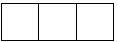
\includegraphics{figures/straight_trominoe.pdf}%
\end{picture}%
\setlength{\unitlength}{3947sp}%
%
\begingroup\makeatletter\ifx\SetFigFont\undefined%
\gdef\SetFigFont#1#2#3#4#5{%
  \reset@font\fontsize{#1}{#2pt}%
  \fontfamily{#3}\fontseries{#4}\fontshape{#5}%
  \selectfont}%
\fi\endgroup%
\begin{picture}(924,324)(1189,-673)
\end{picture}%
 and L-shaped 
\begin{picture}(0,0)%
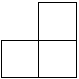
\includegraphics{figures/L-shaped_trominoe.pdf}%
\end{picture}%
\setlength{\unitlength}{3947sp}%
%
\begingroup\makeatletter\ifx\SetFigFont\undefined%
\gdef\SetFigFont#1#2#3#4#5{%
  \reset@font\fontsize{#1}{#2pt}%
  \fontfamily{#3}\fontseries{#4}\fontshape{#5}%
  \selectfont}%
\fi\endgroup%
\begin{picture}(624,624)(1189,-673)
\end{picture}%
. This problem is only concerned with
the L-shaped trominoes.)
\end{enumerate}

\item Suppose that the rules of the game for PMI were changed so that one
did the following:
\begin{itemize}
\item Basis.  Prove that $P(0)$ is true.
\item Inductive step.  Prove that for all $k$, $P_k$ implies $P_{k+2}$
\end{itemize}

\noindent Explain why this would not constitute a valid proof that $P_n$ holds 
for all natural numbers $n$. 
\noindent How could we change the basis in this outline to obtain a valid proof?

\end{enumerate}


%% Emacs customization
%% 
%% Local Variables: ***
%% TeX-master: "GIAM-hw.tex" ***
%% comment-column:0 ***
%% comment-start: "%% "  ***
%% comment-end:"***" ***
%% End: ***




 
\newpage

\section{Formulas for sums and products}


\noindent{\large \bf Exercises --- \thesection\ }

\begin{enumerate}
\item Write an inductive proof of the formula for the sum 
of the first $n$ cubes.

\item Find a formula for the sum of the first $n$ fourth powers.

\item The sum of the first $n$ natural numbers is sometimes called
the $n$-th triangular number \index{triangular numbers}$T_n$.  Triangular numbers are so-named
because one can represent them with triangular shaped arrangements 
of dots. 

\begin{center} \begin{picture}(0,0)%
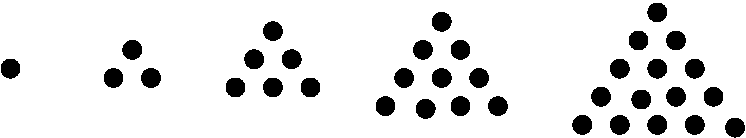
\includegraphics{./triangular_numbers.pdf}%
\end{picture}%
\setlength{\unitlength}{3947sp}%
%
\begingroup\makeatletter\ifx\SetFigFont\undefined%
\gdef\SetFigFont#1#2#3#4#5{%
  \reset@font\fontsize{#1}{#2pt}%
  \fontfamily{#3}\fontseries{#4}\fontshape{#5}%
  \selectfont}%
\fi\endgroup%
\begin{picture}(5963,1088)(1193,-2116)
\end{picture}%
 \end{center}

The first several triangular numbers are 1, 3, 6, 10, 15, et cetera.

Determine a formula for the sum of the first $n$ triangular numbers $\displaystyle \left( \sum_{i=1}^n T_i \right)$ and prove it using PMI.

\item Consider the alternating sum of squares:
\begin{gather*}
1 \\
1 - 4 = -3 \\
1 - 4 + 9 = 6 \\
1 - 4 + 9 - 16 = -10 \\
\mbox{et cetera}
\end{gather*}
Guess a general formula for $\sum_{i=1}^n (-1)^{i-1} i^2$, and prove it using PMI.

\item Prove the following formula for a product.

\[ \prod_{i=2}^n \left(1 - \frac{1}{i}\right) =  \frac{1}{n} \]

\item Prove $\displaystyle \sum_{j=0}^{n}(4j+1) \; = \; 2n^{2}+3n+1$ for all
integers $n \geq 0$.

\item Prove $\displaystyle \sum_{i=1}^{n}\frac{1}{(2i-1)(2i+1)} \; = \; \frac{n}{2n+1}$ for all natural numbers $n$.

\item The \index{Fibonacci numbers} \emph{Fibonacci numbers} are a sequence of integers defined by
the rule that a number in the sequence is the sum of the two that 
precede it.

\[ F_{n+2} = F_n + F_{n+1}  \]

\noindent The first two Fibonacci numbers (actually the zeroth and the first) 
are both 1.  

\noindent Thus, the first several Fibonacci numbers are

\[ F_0 = 1, F_1=1, F_2=2, F_3=3, F_4=5, F_5=8, F_6=13, F_7=21, \; \mbox{et cetera} \]

Use mathematical induction to prove the following formula involving
Fibonacci numbers.

\[ \sum_{i=0}^n (F_i)^2 \, = \, F_n \cdot F_{n+1} \]

\end{enumerate}

%% Emacs customization
%% 
%% Local Variables: ***
%% TeX-master: "GIAM-hw.tex" ***
%% comment-column:0 ***
%% comment-start: "%% "  ***
%% comment-end:"***" ***
%% End: ***



\newpage

\section[Other proofs using PMI]{Divisibility statements and other proofs using PMI}


\noindent{\large \bf Exercises --- \thesection\ }


Give inductive proofs of the following 
\begin{enumerate}
\item $\forall x \in \Naturals, \; 3 \divides x^3-x$

\item $\forall x \in \Naturals, \; 3 \divides x^3+5x$

\item $\forall x \in \Naturals, \; 11 \divides x^{11}+10x$

\item $\forall n \in \Naturals, \; 3 \divides 4^n-1$

\item $\forall n \in \Naturals, \; 6 \divides (3n^{2}+3n-12)$

\item $\forall n \in \Naturals, \; 5 \divides (n^{5}-5n^{3}+14n$

\item $\forall n \in \Naturals, \; 4 \divides (13^{n}+4n-1)$

\item $\forall n \in \Naturals, \; 7 \divides 8^n+6$

\item $\forall n \in \Naturals, \; 6 \divides 2n^3 - 2n - 14$

\item $\forall n \geq 3 \in \Naturals, \; 3n^2+3n+1 < 2n^3$

\item $\forall n > 3 \in \Naturals, \; n^3 < 3^n$

\item $\forall n \geq 3 \in \Naturals, \; n^{3}+3>n^{2}+3n+1$

\item $\forall x \geq 4 \in \Naturals, \; x^22^x \leq 4^x$
\end{enumerate}


%% Emacs customization
%% 
%% Local Variables: ***
%% TeX-master: "GIAM-hw.tex" ***
%% comment-column:0 ***
%% comment-start: "%% "  ***
%% comment-end:"***" ***
%% End: ***



\newpage
 
\section{The strong form of mathematical induction}

\noindent{\large \bf Exercises --- \thesection\ }


Give inductive proofs of the following 
\begin{enumerate}
\item A ``postage stamp problem'' is a problem that (typically) asks
us to determine what total postage values can be produced using two
sorts of stamps.  Suppose that you have $3$\cents\  stamps and $7$\cents\ 
stamps, show (using strong induction) that any postage value $12$\cents\ 
or higher can be achieved.  That is, 

\[ \forall n \in \Naturals, n \geq 12 \; \implies \;
\exists x,y \in \Naturals , n = 3x + 7y. \]
 
\item Show that any integer postage of $12 \cents$ or more can be made using
only $4\cents$ and $5\cents$ stamps.

\item The polynomial equation $x^2 = x+1$ has two solutions, 
$\alpha = \frac{1+\sqrt{5}}{2}$ and $\beta = \frac{1-\sqrt{5}}{2}$.
Show that the Fibonacci number $F_n$ is less than or equal to $\alpha^{n}$
for all $n \geq 0$.

\end{enumerate}


%% Emacs customization
%% 
%% Local Variables: ***
%% TeX-master: "GIAM-hw.tex" ***
%% comment-column:0 ***
%% comment-start: "%% "  ***
%% comment-end:"***" ***
%% End: ***




%% Emacs customization
%% 
%% Local Variables: ***
%% TeX-master: "GIAM-hw.tex" ***
%% comment-column:0 ***
%% comment-start: "%% "  ***
%% comment-end:"***" ***
%% End: ***

